\documentclass[tikz,border=2pt]{standalone}
\usepackage{times}
\usepackage{amsmath}
\begin{document}
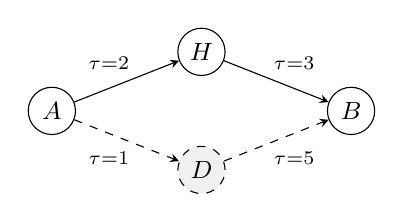
\begin{tikzpicture}[>=stealth,font=\small,
  every node/.style={circle,draw,minimum size=6mm,inner sep=1pt},
  nv/.style={circle,draw,dashed,fill=gray!12,minimum size=6mm,inner sep=1pt}]
\node (A) at (0,0) {$A$};
\node (H) at (1.9,0.75) {$H$};
\node[nv] (D) at (1.9,-0.75) {$D$};
\node (B) at (3.8,0) {$B$};
\draw[->] (A) -- node[above left,draw=none,font=\scriptsize]{$\tau{=}2$} (H);
\draw[->] (H) -- node[above right,draw=none,font=\scriptsize]{$\tau{=}3$} (B);
\draw[->,dashed] (A) -- node[below left,draw=none,font=\scriptsize]{$\tau{=}1$} (D);
\draw[->,dashed] (D) -- node[below right,draw=none,font=\scriptsize]{$\tau{=}5$} (B);
\end{tikzpicture}
\end{document}
